\chapter{Wykorzystane technologie}

\section{Xcode i Developer Tools}
Xcode jest IDE (Integrated development environment) stworzonym przez Apple i dostępnym za darmo do pobrania z App Store, sklepu
z aplikacjami do którego dostęp mają wyłącznie użytkownicy komputerów z systemem MacOS. Jest wyposażony w pakiet wszystkich narzędzi
(Developer Tools) potrzebnych dla developerów aby tworzyć aplikacje na iOS. Główną aplikacją pakietu jest Xcode IDE który wraz z
wspomagającymi aplikacjami dostępnymi w pakiecie takimi jak Simulator czy Instruments czyni pracę przy tworzeniu aplikacji płynną
i efektowną. W tym rozdziale przedstawię właśnie te narzędzia ze względu na ich rolę w procesie tworzenia aplikacji.

\begin{figure}[ht!]
  \centering
  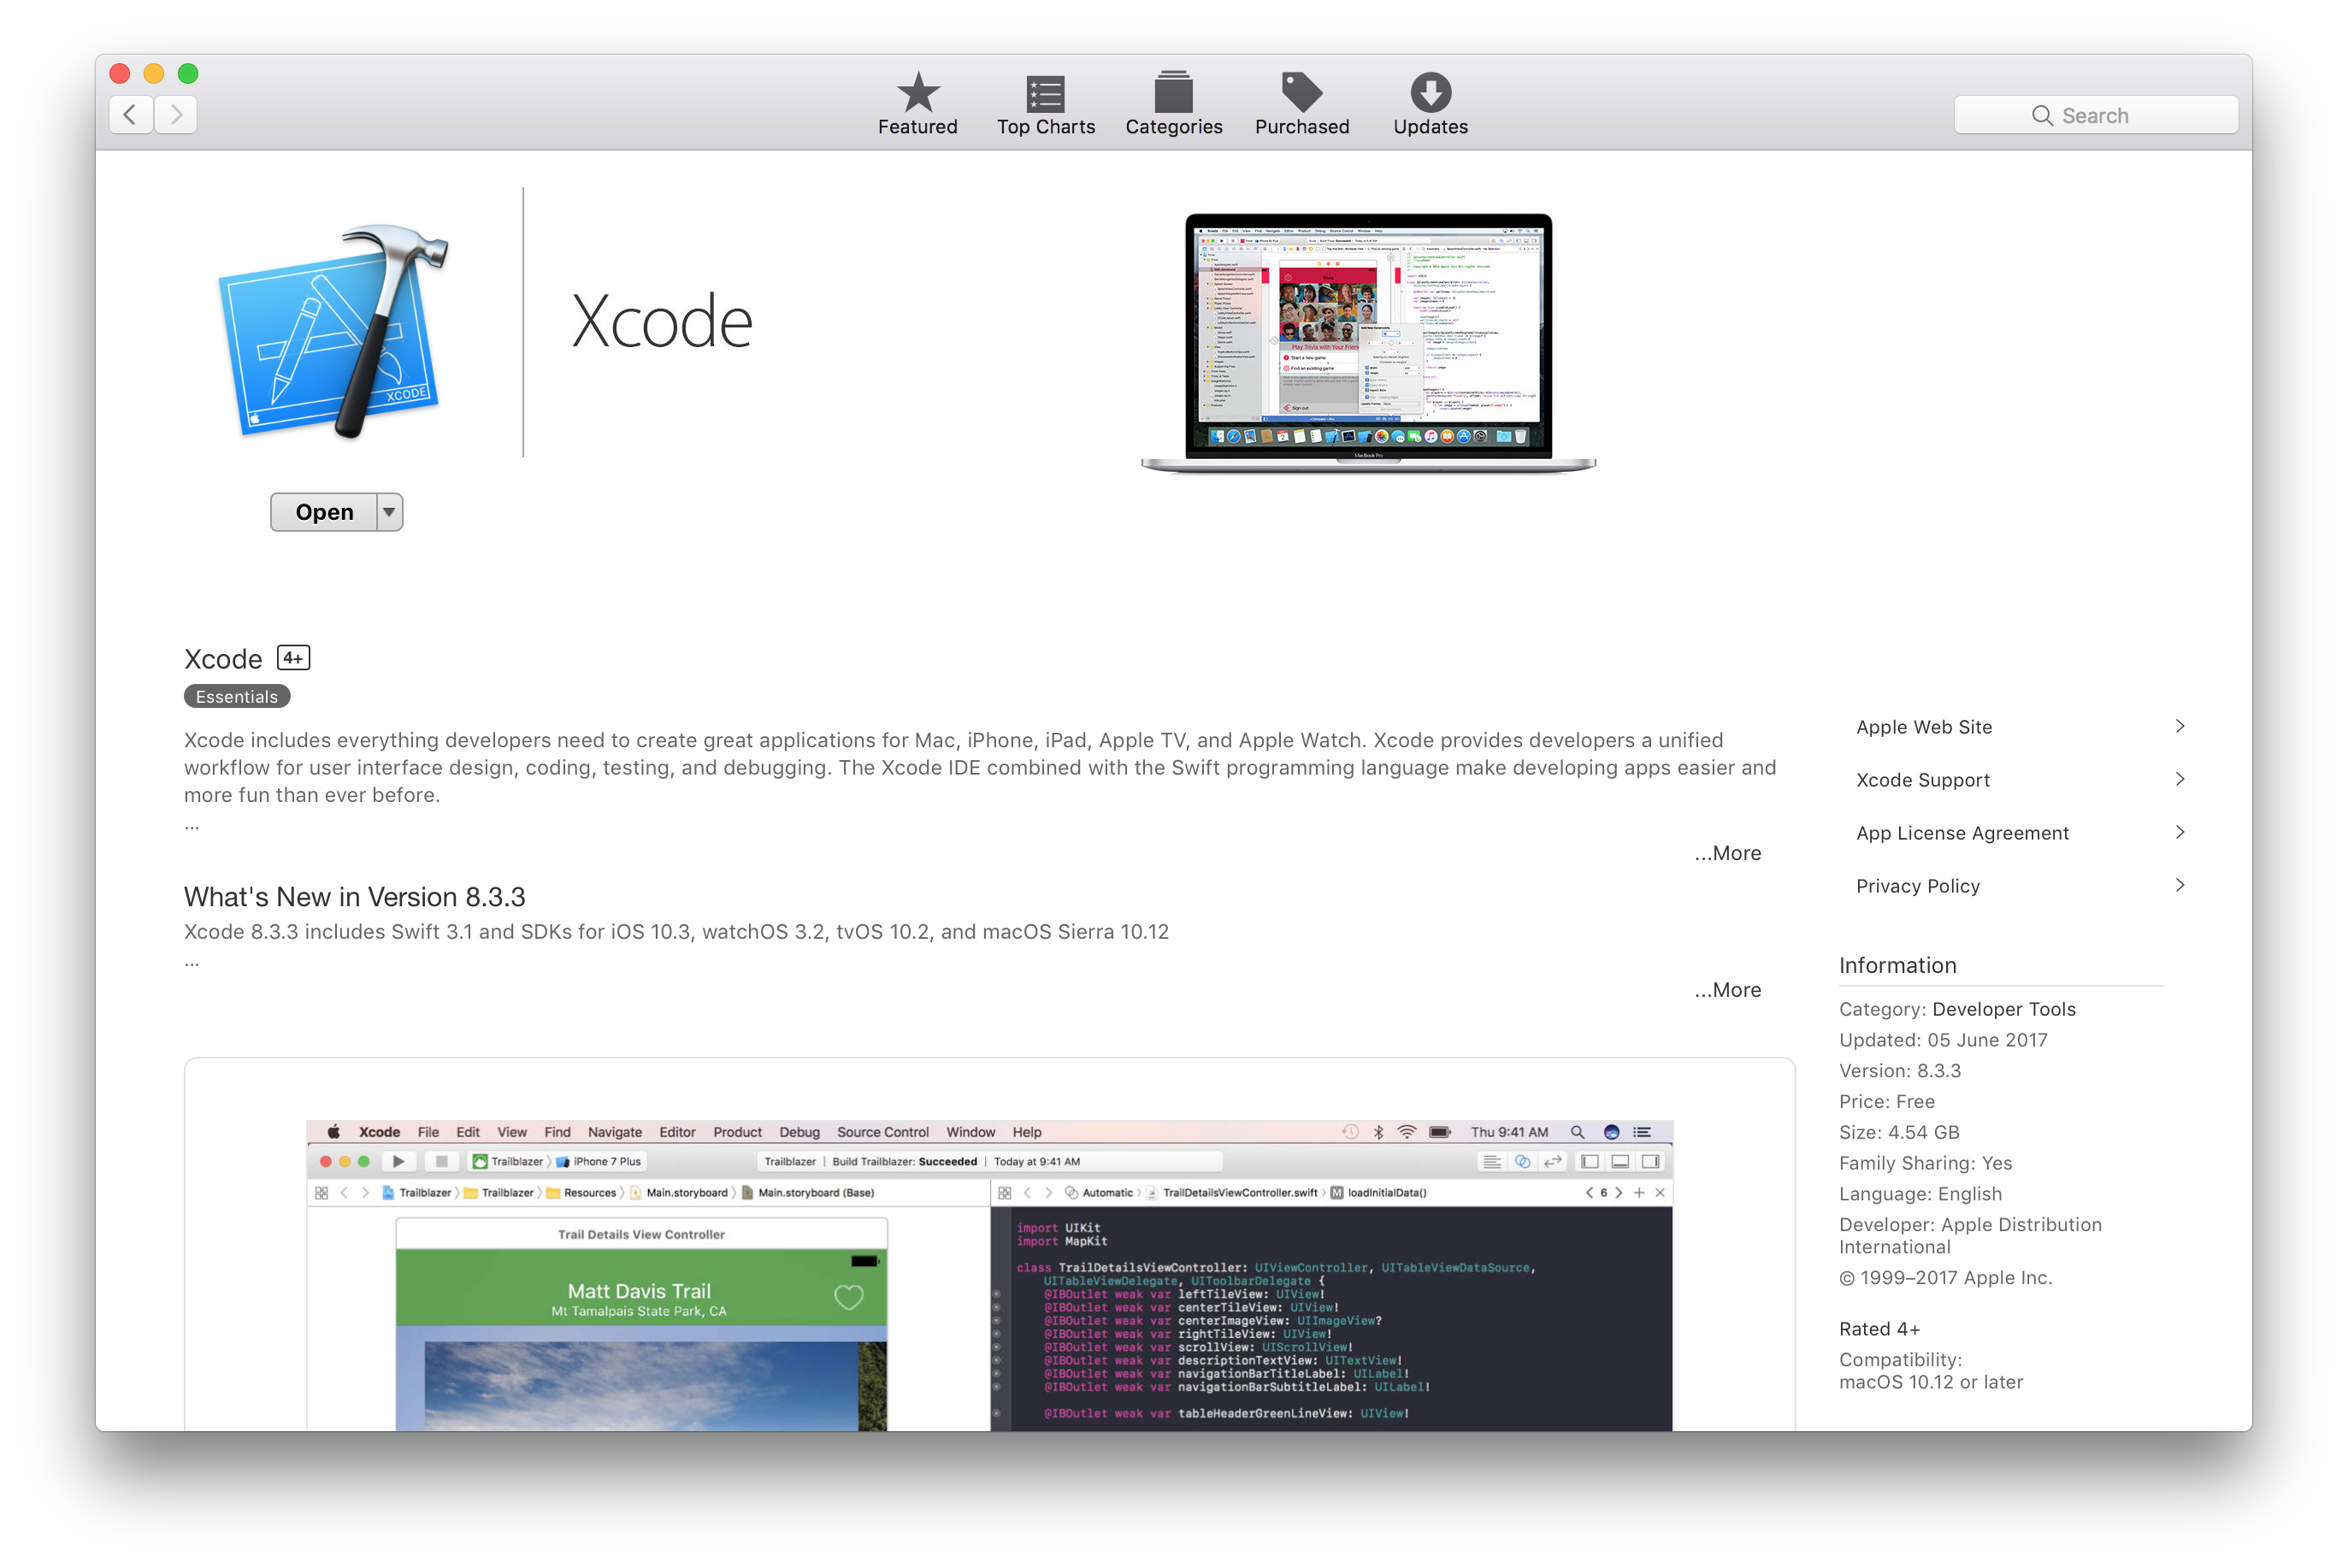
\includegraphics[width=120mm]{images/chapter-2-image-1-appstore.png}
  \caption{Xcode w App Store}
  \label{chapter-2-image-1-appstore}
\end{figure}

\subsubsection*{Xcode IDE}
Xcode jako nowoczesne, produktywne środowisko jest miejscem w którym programista aplikacji na iOS spędza większość swojego
czasu. Całość prac wykonywanych przy produkcji aplikacji może zostać wykonana właśnie tutaj. Najbardziej podstawowy element jakim
jest edytor tekstu dobrze współgra z takimi narzędziami jak Interface Buildier, który pozwala w prosty sposób zaprojektować stronę
wizualną aplikacji przy użyciu Storyboardów a następnię stworzyć referencję w kodzie do wybranych przez nas elementów przez proste
przeciągnięcie myszką. Storyboardy są opcjonalnym aczkolwiek bardzo pożytecznym narzędziem szczególnie dla programistów stawiających
swoje pierwsze kroki na tej platformie. Zapewniają one wizualne wyobrazenie interfejsu aplikacji nad którą wykonywana jest praca,
a projektowanie dowolnego widoku który będzie wyglądał dobrze na każdym urządzeniu w dowolnej orientacji, jest relatywnie proste po
zapoznaniu się z kilkoma elementarnymi zasadami.

\begin{figure}[ht!]
  \centering
  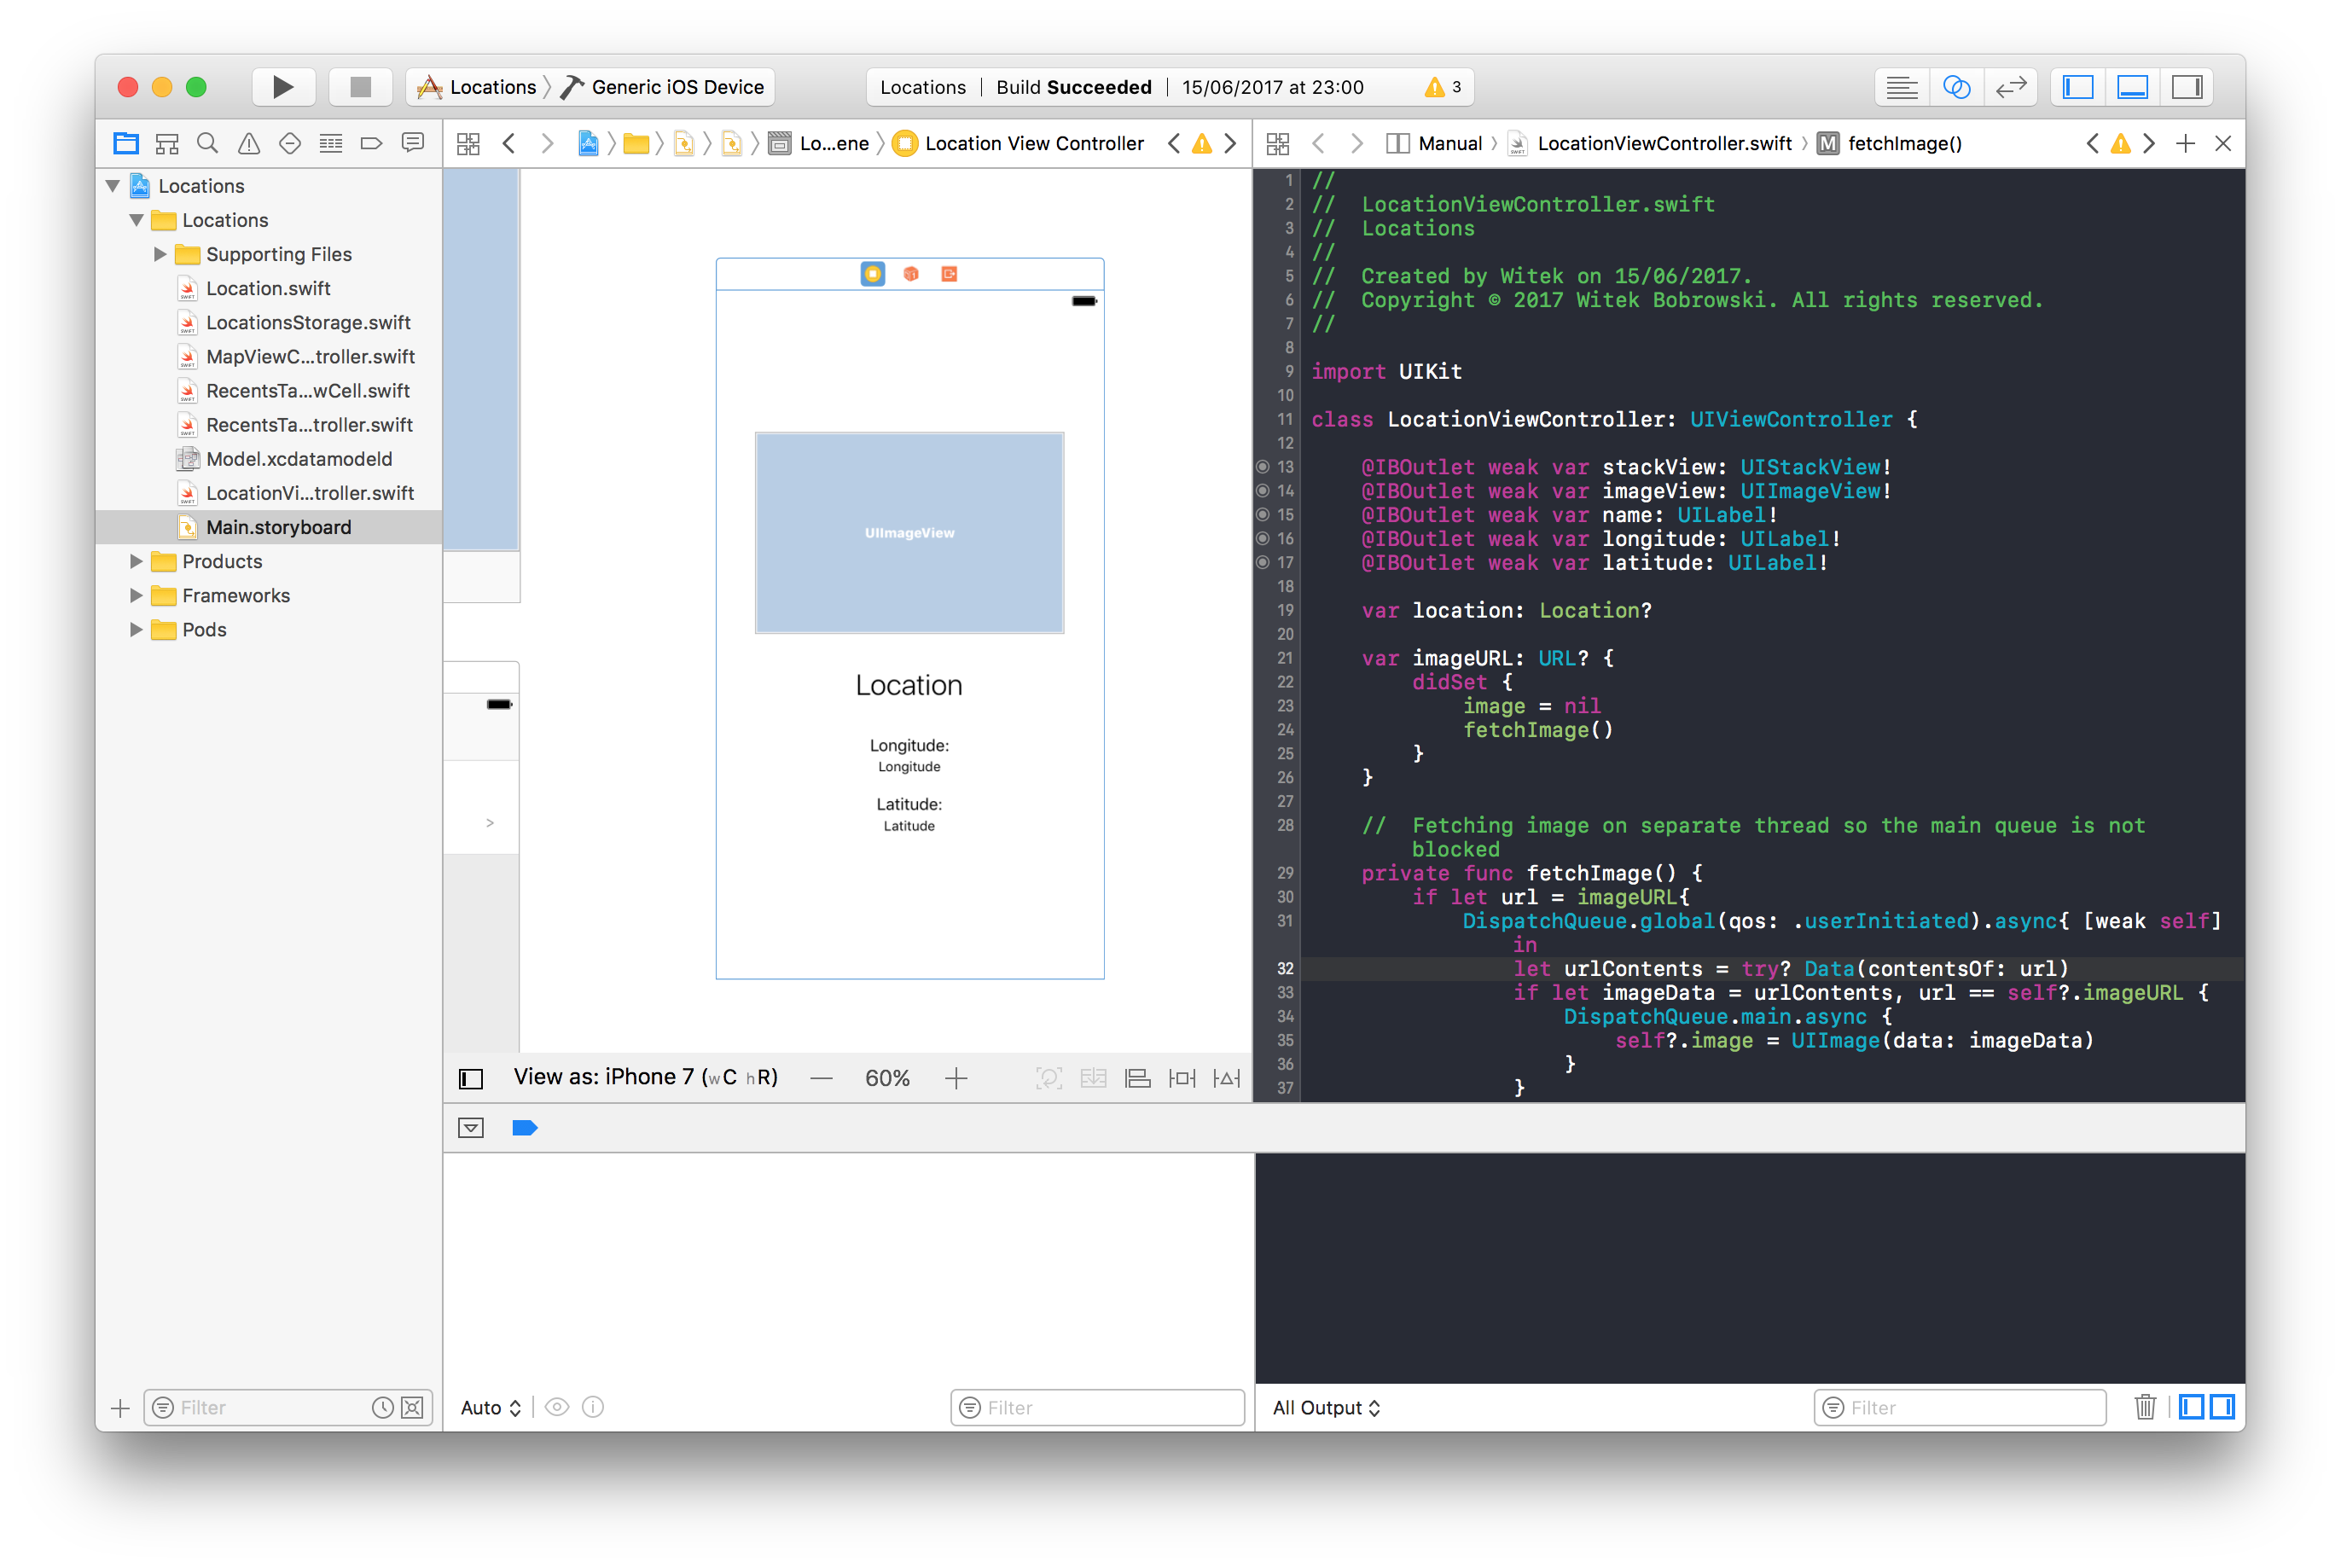
\includegraphics[width=120mm]{images/chapter-2-image-2-xcode.png}
  \caption{Xcode pokazujący "Assistant editor"}
  \label{chapter-2-image-2-xcode}
\end{figure}

Ponieważ Storyboardy tworzy się w jednym pliku o formacie .storyboard, często w profesjonalnej produkcji rezygnuje się z nich ze
względu na konflikty w systemach kontrolii wersji. Konflikty te powstają w wyniku pracy wielu programistów, a ponieważ plik .storyboard
jest w rzeczywistości plikiem XML, który został wygenerowany automatycznie, rozwiązywanie konfilków bywa kłopotliwe, a przy dużych
projektach problematyczne. Dlatego rezygnuje się z nich na rzecz tworzenia widoków tylko przy użyciu kodu, oraz niezależnych plików XIB.
Pliki te pozwalają na ustawienie elementów w stylu znanym ze Storyboardów lecz w przeciwieństwie do nich reprezentrują pojedyńczy widok,
dzięki czemu problem z konfliktami zostaje uniknięty a jednocześnie tworzenie bardziej skomplikowanych widoków pozostaje znacznie
ułatwione.
Xcode zapewnia wsparcie dla systemu kontroli wersji git. Przy tworzeniu nowego projektu, gdy jest o to poproszony, inicjalizuje nowe
repozytorium. Dodatkowo w nawigatorze projektu, w którym widać strukturę projektu, Xcode oznaczy literą "M" pliki które git oznacza
jako pliki w których dokonano zmian (modified) a literą "A" pliki które zostały dodane (new file) od czasu poprzedniego zachowania zmian.
W najnowszej wersji 9.0, Xcode zyskał nową funkcjonalność - Source Control Navigator, który pozwala na eksplorowanie poszczególnych
gałęzi repozytorium i podglądu dowolnego momentu w jego historii.

\subsubsection*{Simulator}
Simulator pozwala na uruchomienie zbudowanej aplikacji na dowolnym urządzeniu z iOS które jest w stanie zasymulować. Gdy chce się
przetestować aplikację wystarczy w pasku narzędzi Xcode wybrać dowolny model urządzenia (oprócz telefonów iPhone znajdują się tam
rówież tablety iPad) które chcemy zasymulować (jeżeli podłączymy do komputera fizyczne urządzenie, Xcode rówiez je wykryje i pozwoli
na zainstalowanie i uruchomienie na nim aplikacji), a Xcode przejdzie to etapu budowania aplikacji w którym kompiluje pliki źródłowe,
a następnie umieści aplikację w symulatorze wybranego przez nas urządzenia.

\begin{figure}[ht!]
\centering
\begin{subfigure}{.5\textwidth}
  \centering
  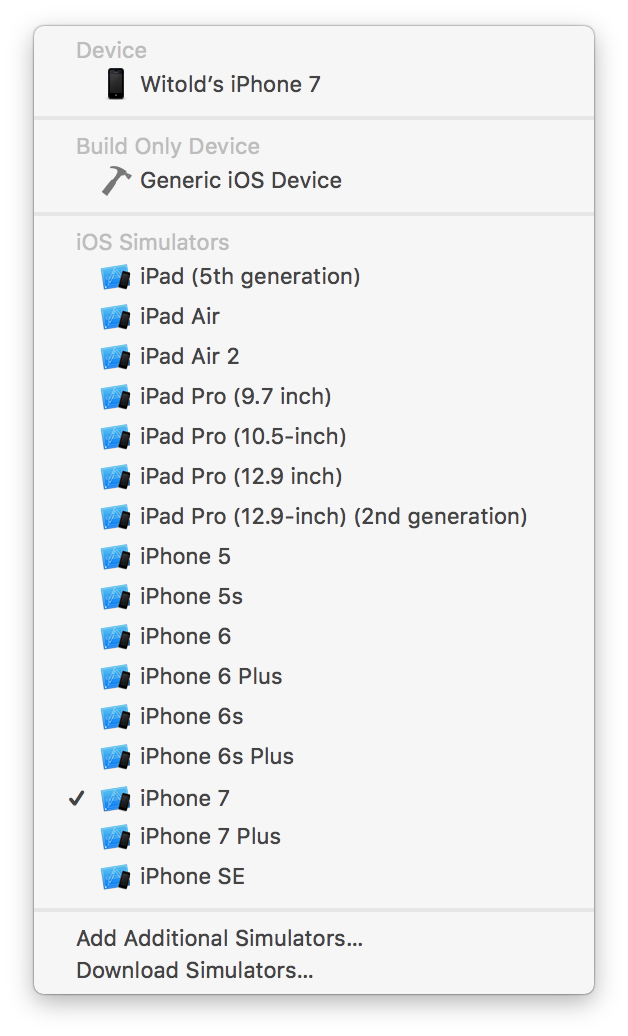
\includegraphics[width=.4\linewidth]{images/chapter-2-image-3-target.png}
  \caption{Wybór docelowego urządzenia}
  \label{chapter-2-image-3-target}
\end{subfigure}%
\begin{subfigure}{.5\textwidth}
  \centering
  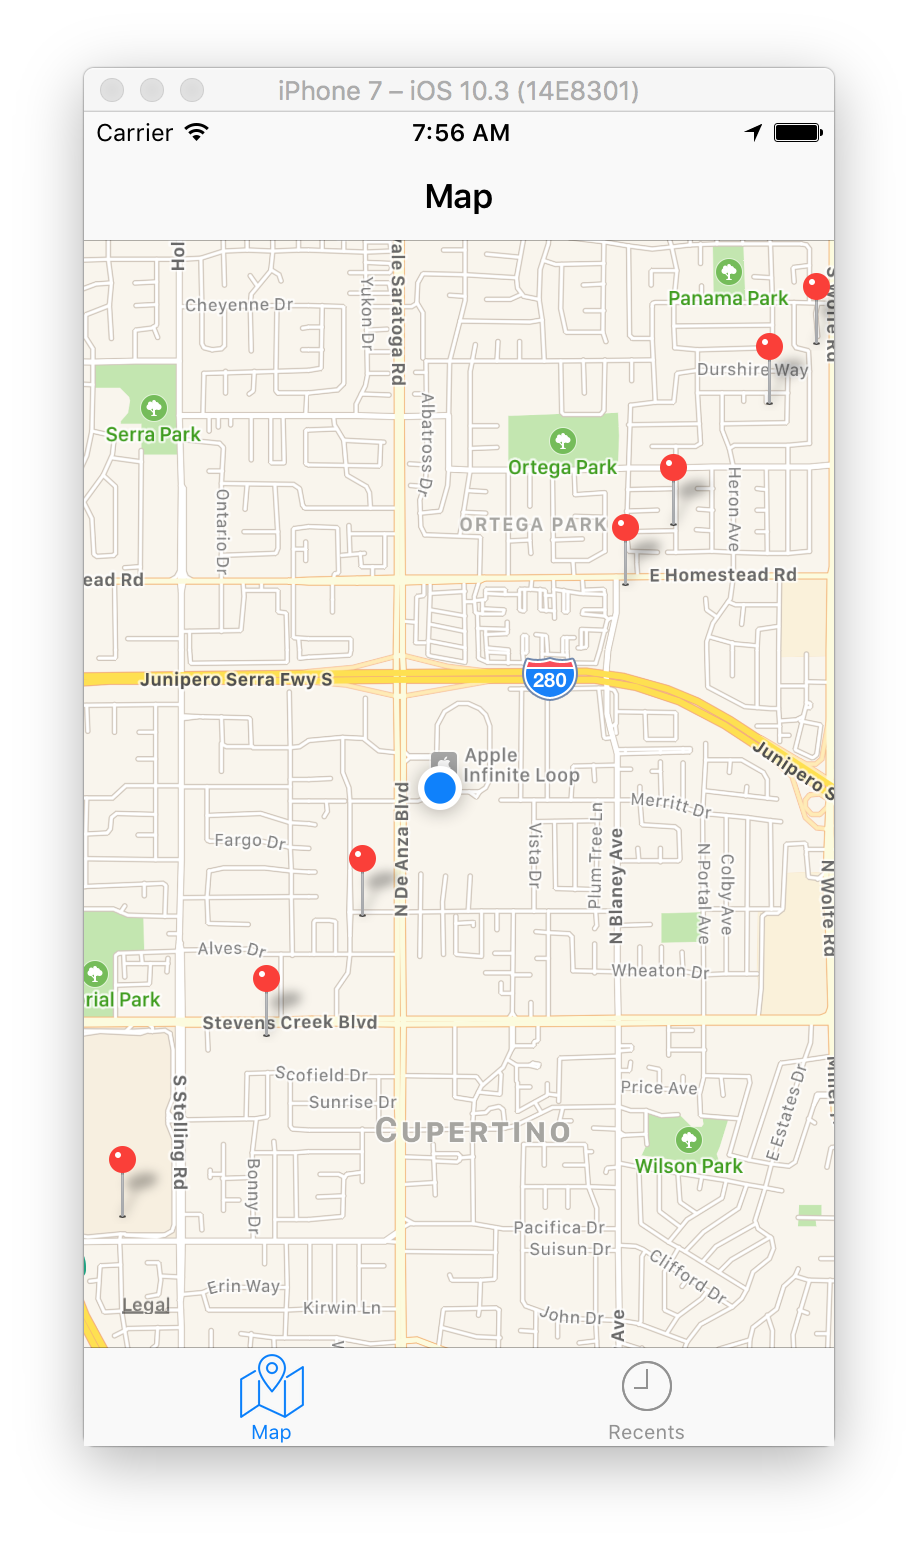
\includegraphics[width=.4\linewidth]{images/chapter-2-image-4-simulator.png}
  \caption{Uruchomiona aplikacja na iPhone 7}
  \label{chapter-2-image-4-simulator}
\end{subfigure}
\caption{Po wybraniu urządzenia w Xcode, Simulator uruchamia na nim aplikację}
\label{chapter-2-image-4-5}
\end{figure}

Podczas gdy aplikacja jest uruchomiona i testowana na symulatorze, Xcode pozwala na podgląd użycia zasobów takich jak procesor, pamięć
RAM, pamięć dyskowa oraz sieć. Po wybraniu dowolnego z wyżej wymienionych zasobów z nawigatora Debuggera ukazje nam się bardziej
szczegółowy podgląd na to w jakim stopniu aplikacja obciąża urządzenie co pozwala na szczegółowe testowanie.

\begin{figure}[ht!]
  \centering
  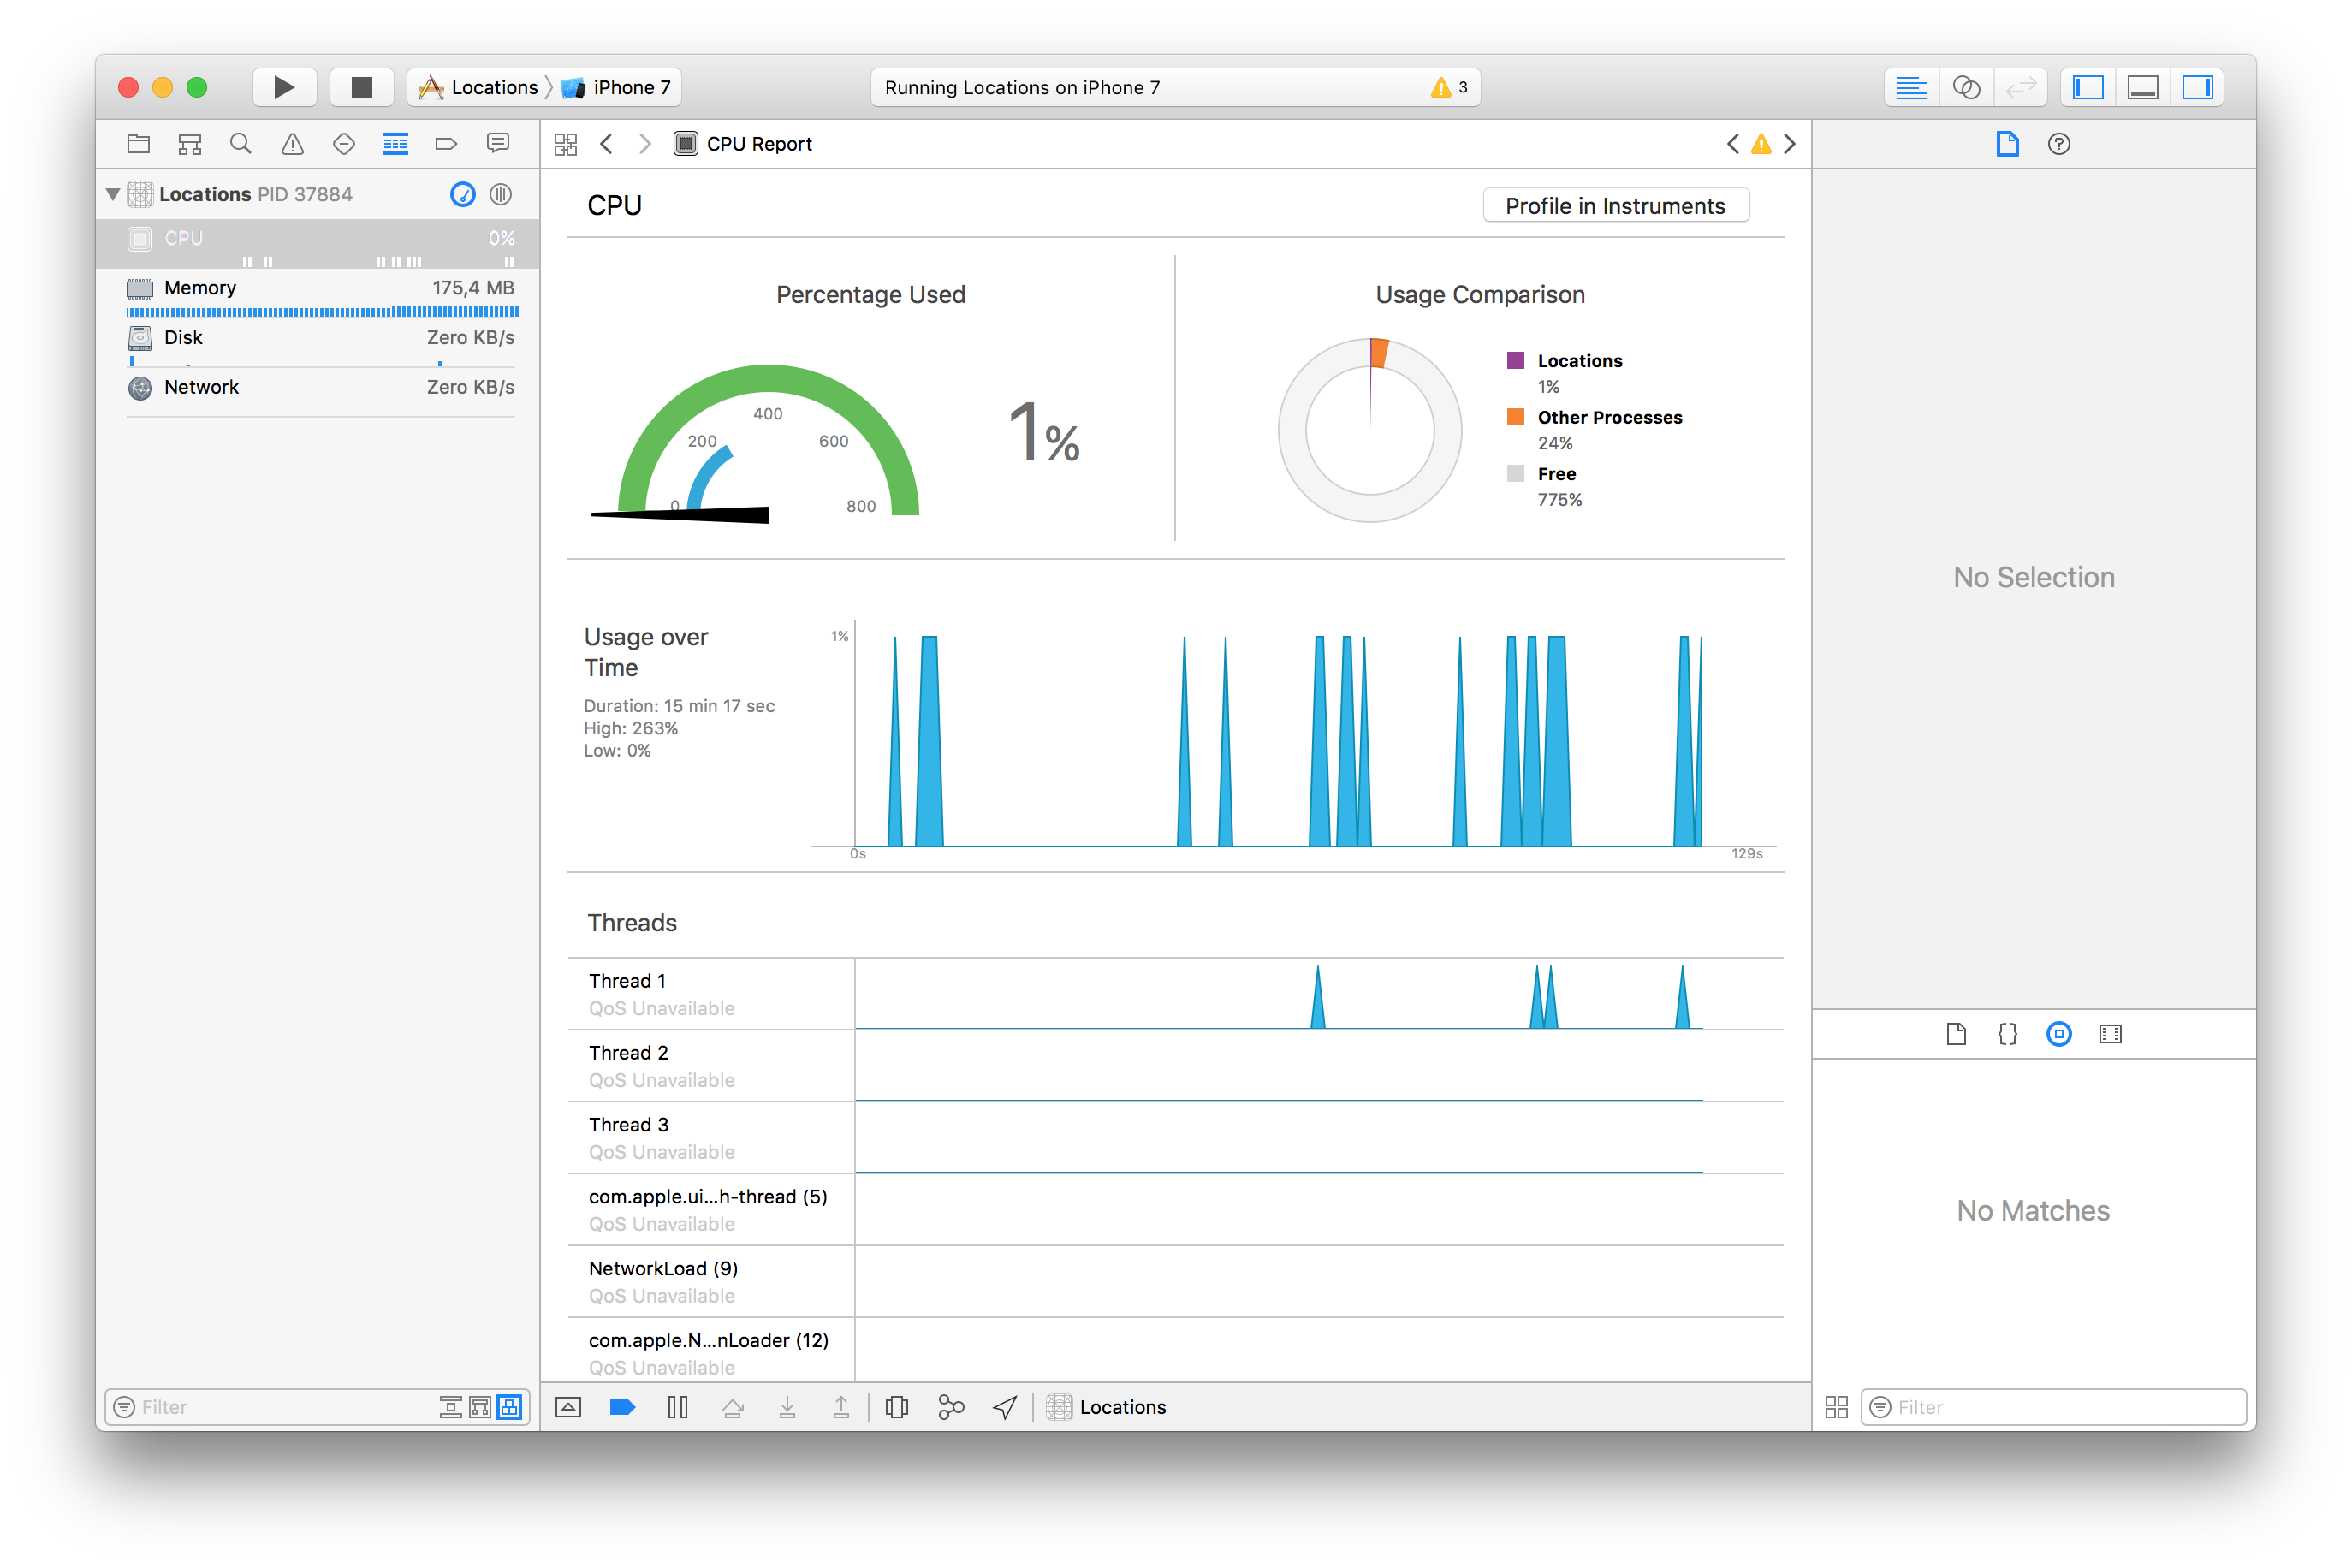
\includegraphics[width=120mm]{images/chapter-2-image-5-debugger.png}
  \caption{Użycie CPU na symulatorze odświeżane na bieżąco i wyświetlne w Xcode}
  \label{chapter-2-image-5-debugger}
\end{figure}

\subsubsection*{Instruments}

Widok poboru zasobów w Xcode jest bardzo pomocny na poglądową ocenę wydajności naszej aplikacji, jeżeli jednak chcemy poddać ją
prawdziwej próbie, musimy uruchomić kolejne narzędzie jakim jest Instruments. Instruments jest aplikacją dzięki której dokonamy
pomiaru nie tylko każdego zasobu na urządzeniu, ale również dostajemy możliwość nadzoru takich aktywności jak alokowanie pamięci
dla obiektów, zmiany layoutu widoków czy zmiany w Core Data, natywnej bazie danych dla iOS.

\begin{figure}[ht!]
  \centering
  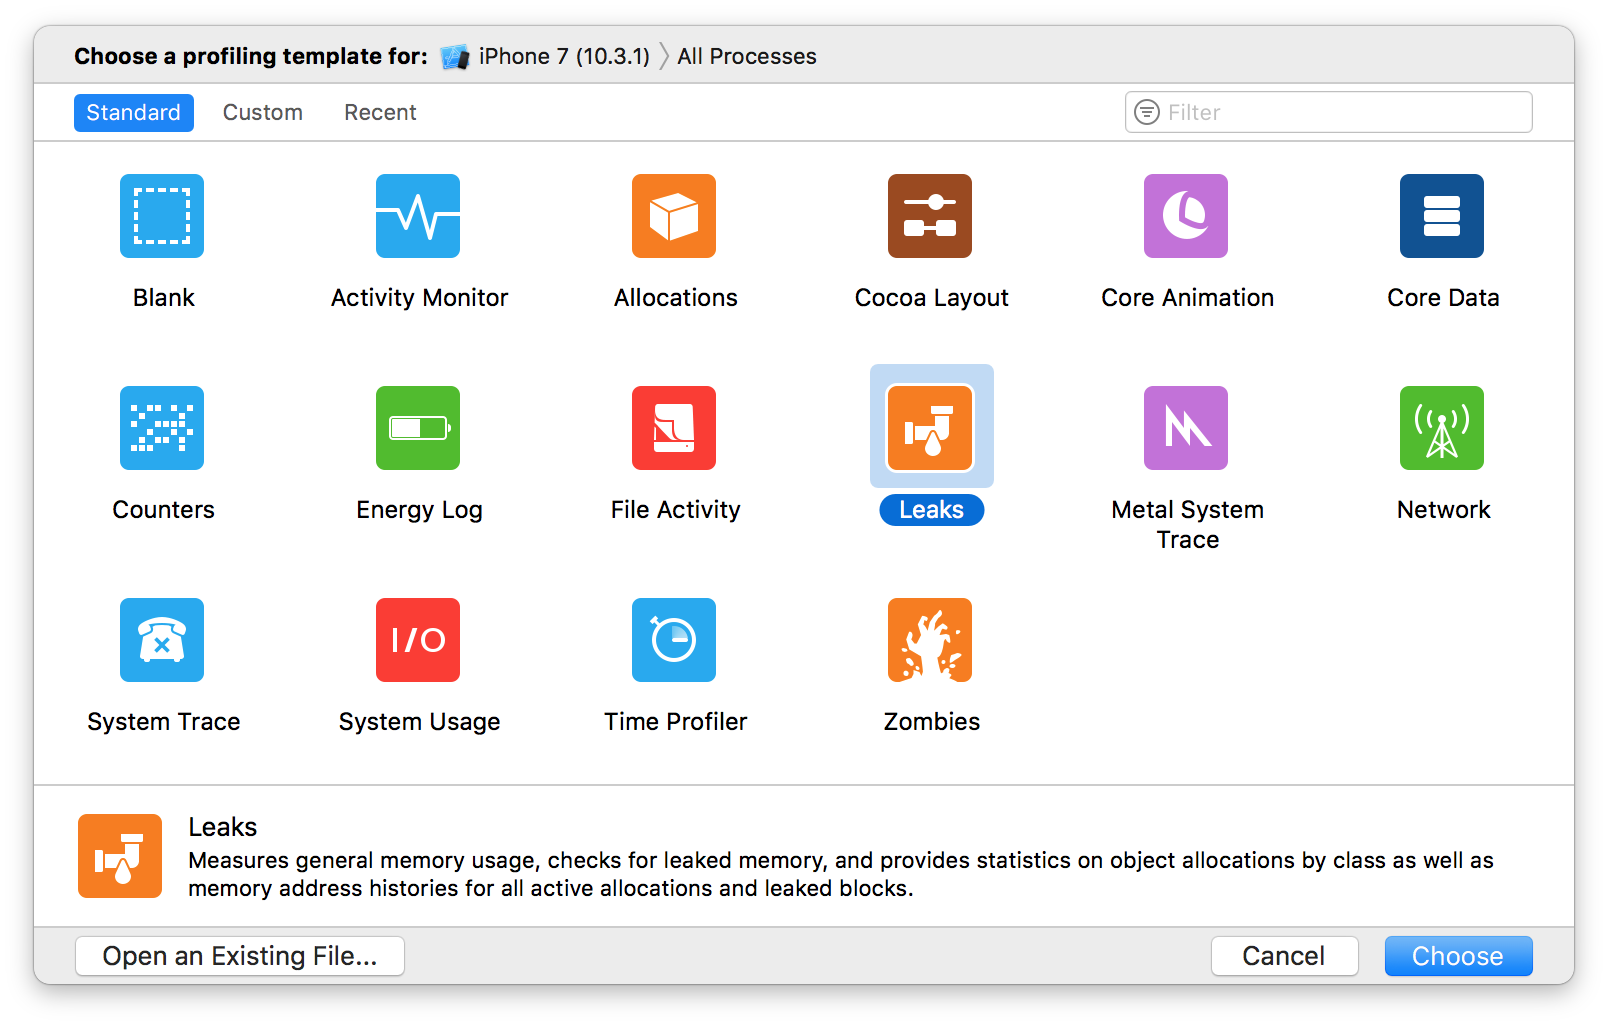
\includegraphics[width=120mm]{images/chapter-2-image-6-instruments.png}
  \caption{Instruments, menu główne}
  \label{chapter-2-image-6-instruments}
\end{figure}

Niezależnie od tego jak szybkie i wydajne są w dzisiejszych czasach telefony, optymalny kod nadal jest podstawą prawidłowego działania
aplikacji i niedbałe projektowanie architektury może być fatalne w skutkach. Cykle referencji mogą powodować niechciane wycieki pamięci
a problemy powstające podczas przerysowywania się widoków spowodują nieczytelny interfejs. Jeżeli takie błędy nie zostaną wykryte na
etapie produkcyjnym, a dogłębne testy aplikacji nie zostaną przeprowadzone przed oddaniem jej do recenzji (Aby nasza aplikacja mogła
znależć się w sklepie AppStore, i być dostępna dla każdego, musi ona otrzymać pozytywną recenzje Apple) aplikacja najprawdopodobniej
zostanie odrzucona, co wiąże się z dodatkowymi opóźnieniami. Pakiet narzędzi dostarczanych przez Apple spełnia swoje zadanie i dla
większości developerów są one wystarczające. Istnieją rozwiązania firm trzecich, JetBrains dostarcza alternatywne IDE do produkcji
aplikacji - AppCode, które cieszy się bardzo dobrą reputacją wśród użytkowników.

\section{Swift}

\section{iOS SDK}

\section{Zewnętrzne biblioteki}
